\documentclass[a4paper]{article}

\usepackage{graphicx}
\usepackage{float}
\usepackage{template}


\begin{document}
%----------------------------------------------------------------------------------------
%   Cover
%----------------------------------------------------------------------------------------
\thispagestyle{empty}
\begin{figure}[ht]
\centering

\includegraphics[height=2.75cm]{title.png}
\end{figure}
\begin{center}
\zihao{0}
\textbf{高级语言程序设计大作业开题报告}
\end{center}
\nopagebreak[4]
\begin{center}
\zihao{1}
\ \\
\end{center}
\nopagebreak[4]
\begin{center}
\zihao{2}
\textbf{作业题目：电竞经理}
\end{center}
% Via \quad, \qquad or '\ ' (backslash and space) you can adjust any space

\begin{center}
    \zihao{1}
    \ \\\ \\\ \\
\end{center}
\nopagebreak[4]
\begin{spacing}{1.8}
    \begin{center}
        %\zihao{-3}
        \begin{table}[ht]
            \centering
            \setlength{\tabcolsep}{7mm}{
                \renewcommand\arraystretch{2.5}
                \begin{tabular}{cc}
                    \zihao{-3}学\quad \quad 院 & \zihao{-3}计算机科学与技术          \\ \cline{2-2} 
                    \zihao{-3}专\quad \quad 业 & \zihao{-3}计算机类         \\ \cline{2-2} 
                    \zihao{-3}学生姓名         & \zihao{-3}杨华城\quad 李睿 \quad DAVUDOV SERDAR          \\ \cline{2-2} 
                    \zihao{-3}学生学号         & \zihao{-3}202430451747 \quad 202430450971 \quad 202469990754    \\ \cline{2-2} 
                    \zihao{-3}任课老师         & \zihao{-3}徐红云     \\ \cline{2-2} 
                \end{tabular}
            }
        \end{table}
    \end{center}
\end{spacing}
\pagebreak[4]
\thispagestyle{empty}
\mbox{}


\setboolean{@twoside}{true}
\begin{spacing}{1.5}
\zihao{-4}
\setcounter{page}{1}
\pagenumbering{arabic}

\section{选题背景和意义}
    随着电子竞技产业的蓬勃发展，全球电子竞技市场规模已突破千亿美元，
中国电竞用户规模超5亿人，职业联赛、俱乐部运营、赛事商业化等体系日趋成熟。
电竞行业从“小众娱乐”发展为“全民文化现象”，带动了游戏开发、直播、周边产业等完整生态链。
在年轻人群体中，电子竞技已经成为很多人生活中不可或缺的一部分。从玩竞技游戏，到观看比赛直播，电竞这个词已深入人心，成为年轻人社交的重要一环。

    每一个电竞爱好者都希望能够组建自己的梦之队，实现自己的电竞梦想，我们的选题正是基于这一诉求，让玩家能够组建自己的战队，
通过参加赛事获得资金和积分，使用资金购买更强的选手，提高“世界排名”。

    通过本次课程设计，我们能熟悉C++面向对象的开发流程，了解OOP的优势和设计模式，为以后的软件开发和设计打下坚实的基础。


    \newpage

\section{设计思路}
    首先是基本流程。
    \begin{figure}[H]
        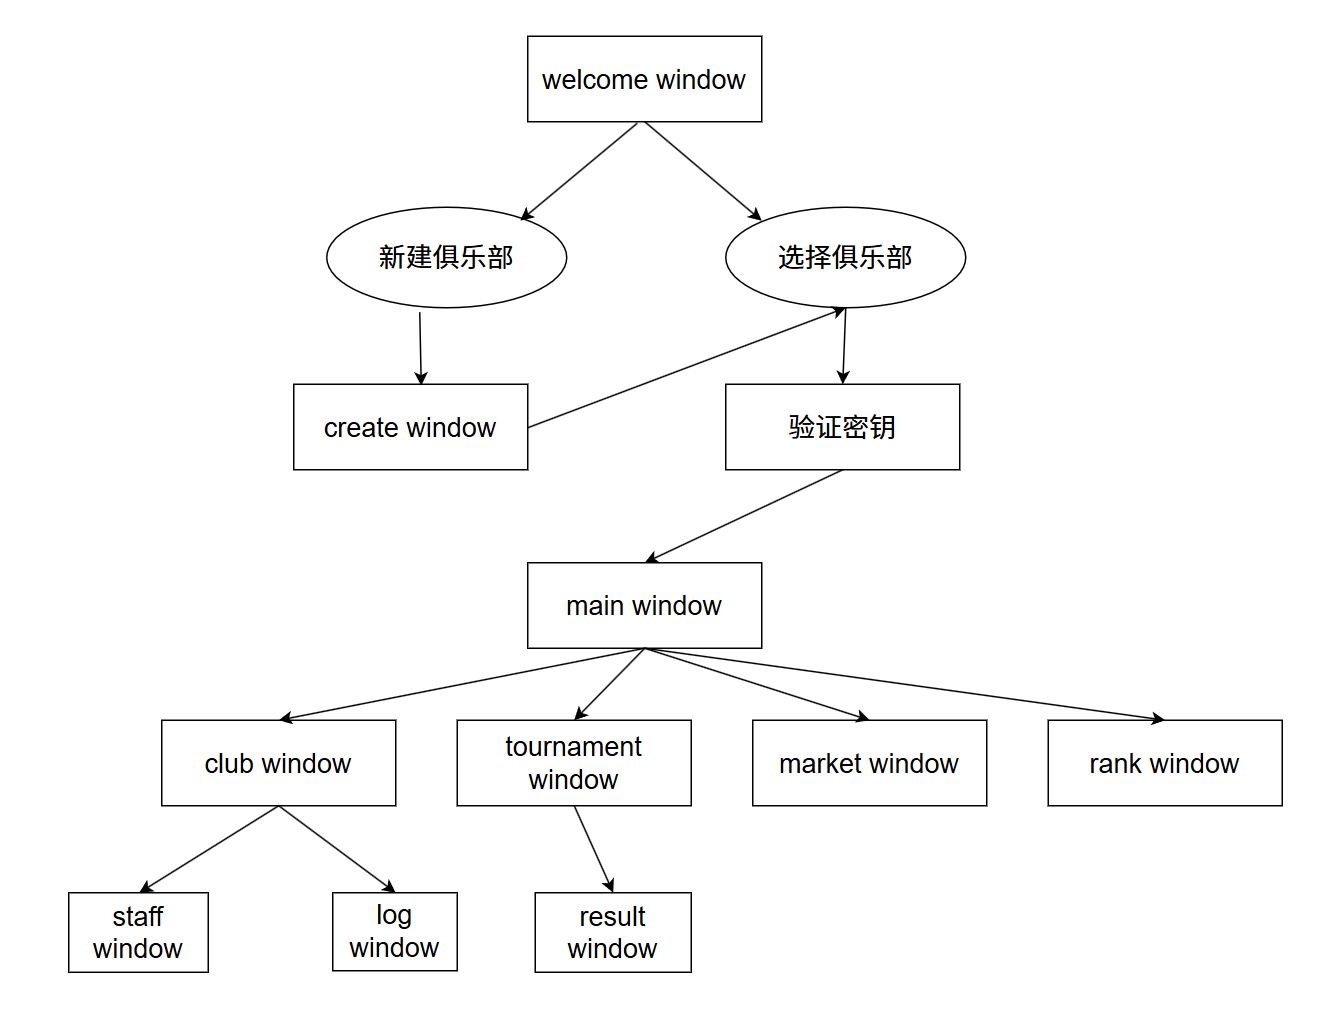
\includegraphics[width=\textwidth]{figure/flowchart/flow chart.png}
        \caption{基本流程图}
    \end{figure}
    整个系统主要由两个主界面组成，分别是welcome界面和main界面。其中welcome界面主要用于用户对俱乐部的选择，而main界面通过一系列子界面满足用户对当前俱乐部的管理。
    
    下面是对上述基本流程图的进一步细分。
    \subsection{欢迎界面}
    \begin{figure}[H]
        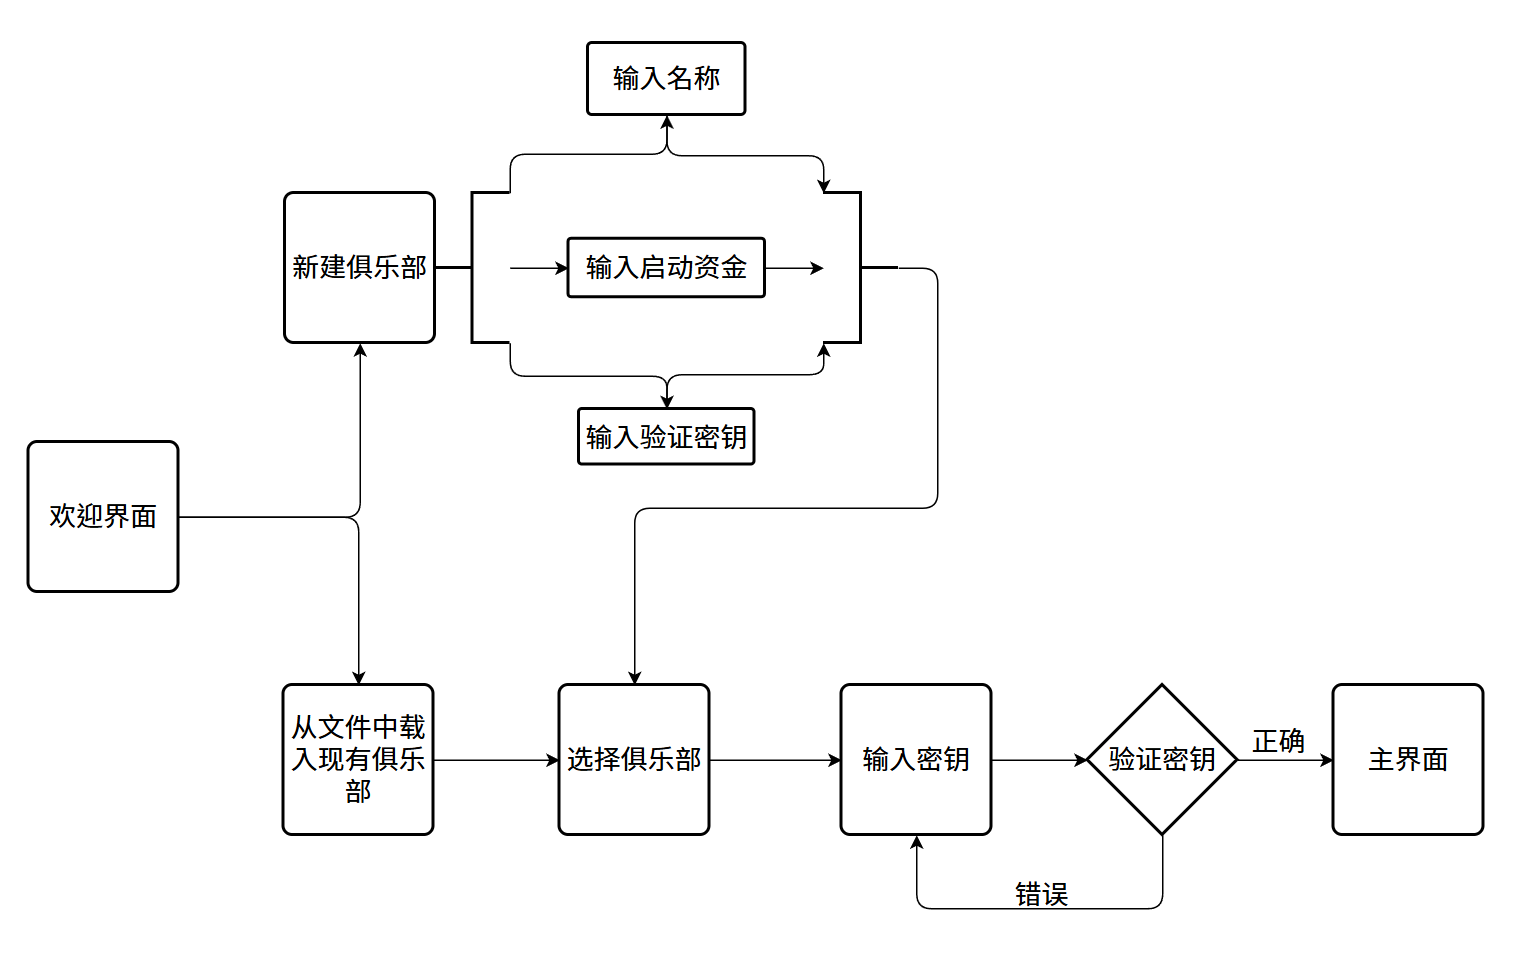
\includegraphics[width=\textwidth]{figure/flowchart/welcome.png}
        \caption{欢迎界面}
    \end{figure}    
    欢迎界面由两大功能模块组成，分别是俱乐部选择和创建，最终引导用户选择目标俱乐部并完成验证，以进入main界面。这里涉及的操作如下：
    \begin{enumerate}
        \item 新建俱乐部：调用Club类的构造函数，并将信息保存到文件中
        \item 载入俱乐部：从文件中读取信息并输出
        \item 选择俱乐部：将目标俱乐部的信息赋值给当前俱乐部
        \item 验证密钥：对比输入和当前俱乐部的密钥
    \end{enumerate}
    
    \subsection{主界面}
    \begin{figure}[H]
        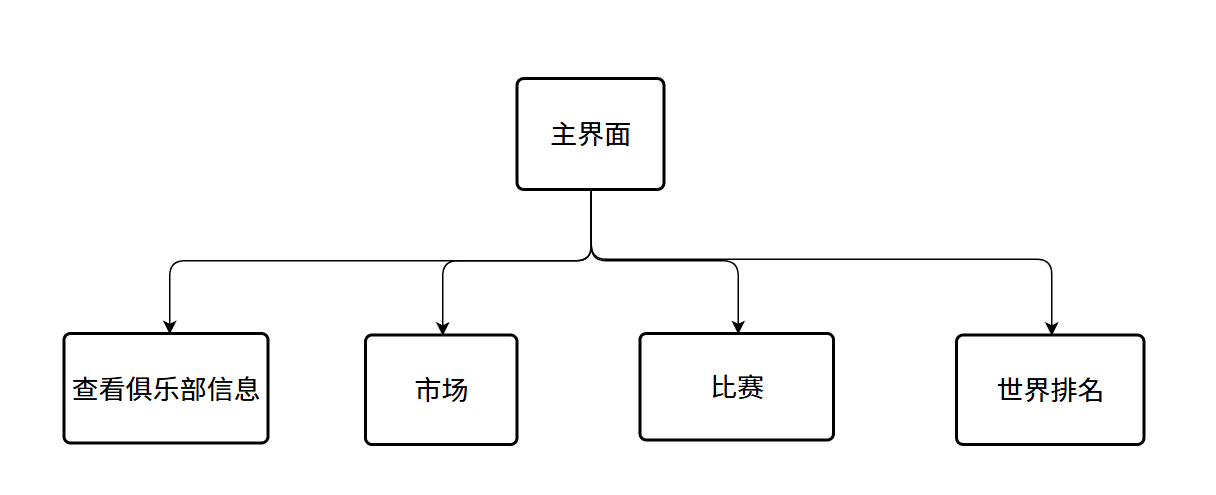
\includegraphics[width=\textwidth]{figure/flowchart/main.png}
        \caption{主界面}
    \end{figure}
    主界面由四大功能模块组成，分别是展示当前俱乐部的信息、市场、比赛和世界排名。下面一一进行介绍。
    
    \subsubsection{俱乐部信息}
    \begin{figure}[H]
        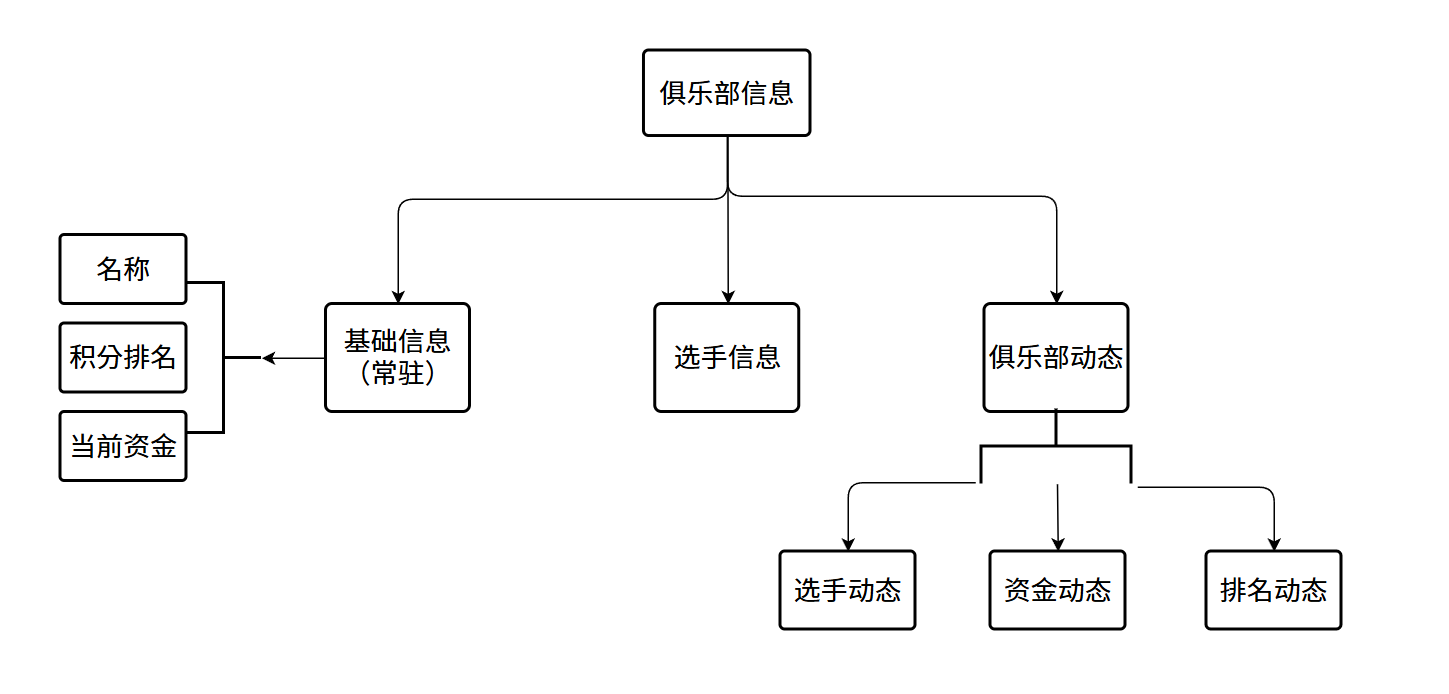
\includegraphics[width=\textwidth]{figure/flowchart/club.png}
        \caption{俱乐部信息}
    \end{figure}
    俱乐部信息分为三大部分，一是常驻信息，即一直会展示的部分信息，包括俱乐部名称、当前的积分和排名，以及当前资金；
    二是选手信息，输出当前俱乐部所拥有的选手信息，包括选手名称、选手位置、选手身价和选手属性（参照HLTV属性对选手一系列的能力进行的评分）；
    三是俱乐部动态，包括选手动态（交易信息）、资金动态和排名动态。

    这部分涉及的主要操作是对当前Club对象的信息的输出。

    \subsubsection{市场}
    \begin{figure}[H]
        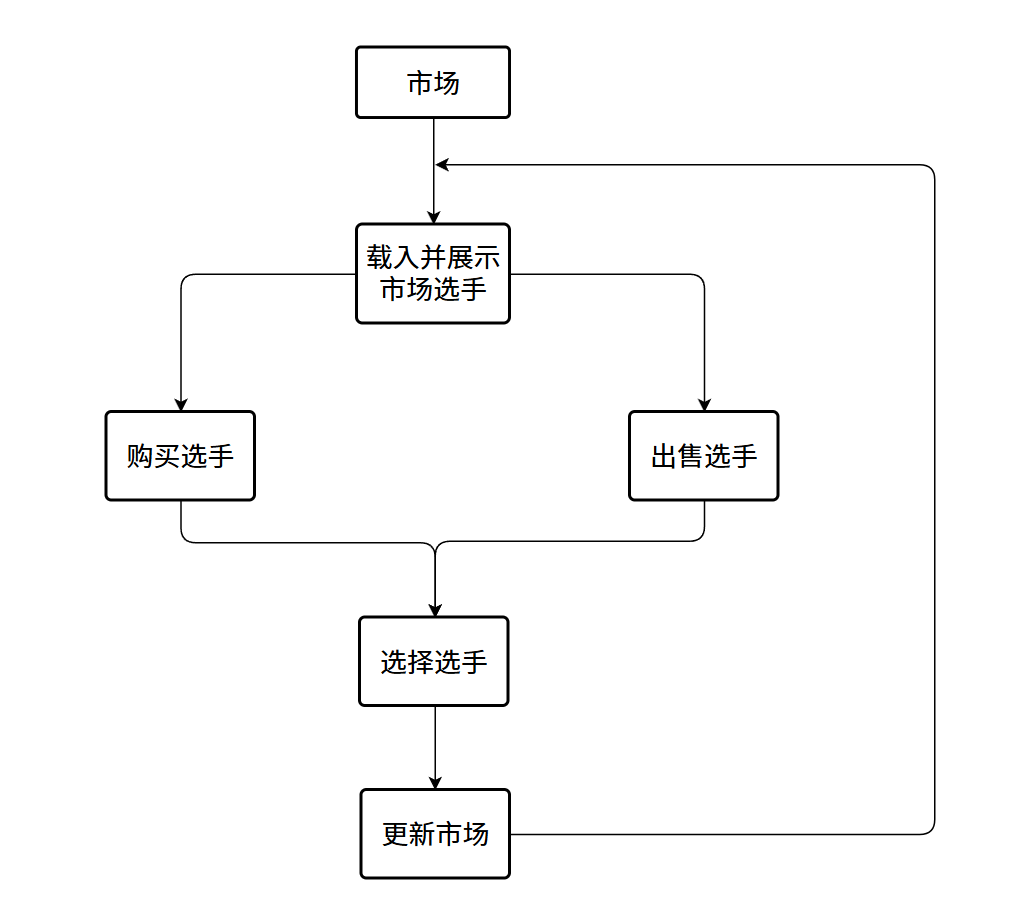
\includegraphics[width=\textwidth]{figure/flowchart/market.png}
        \caption{市场}
    \end{figure}
    在市场界面，首先是对市场选手（无俱乐部归属的选手）的展示；接着用户可以对市场选手进行购买操作，或是对本俱乐部选手进行出售操作；最后更新市场。

    这部分涉及的操作如下：
    \begin{enumerate}
        \item 载入市场并展示：从选手文件中读取state为false的选手，从中随机选择部分加入市场选手列表，并进行输出
        \item 购买选手：引导用户选择市场选手
        \item 出售选手：引导用户选择当前俱乐部选手
        \item 选择选手：将目标选手赋给当前选手
        \item 处理购买出售：改变当前俱乐部的资金，改变当前选手的state和club，并重新储存
        \item 更新市场：移除或添加选手至市场选手
    \end{enumerate}


    \subsubsection{比赛}
    \begin{figure}[H]
        \centering
        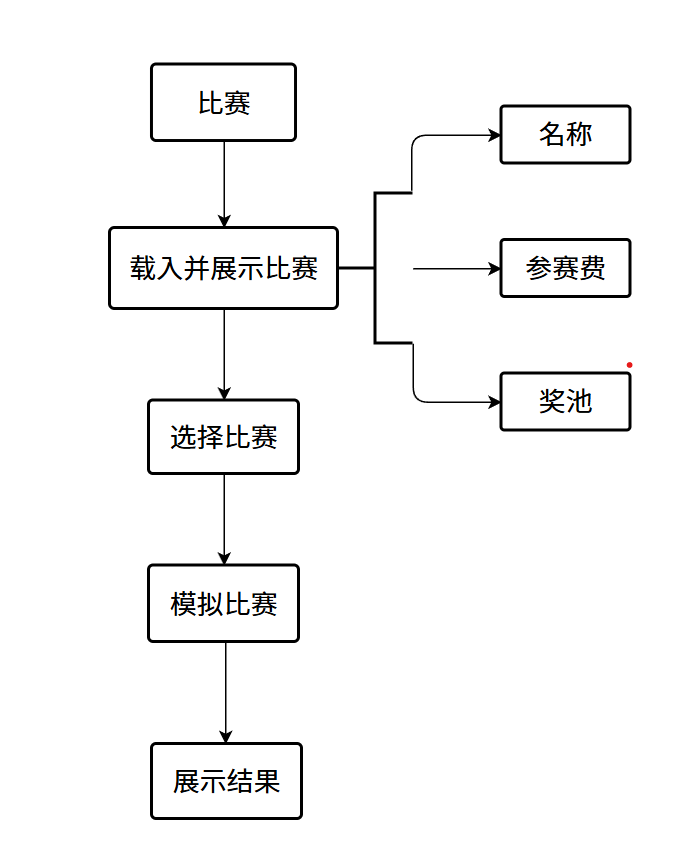
\includegraphics[width=0.8\textwidth]{figure/flowchart/tournament.png}
        \caption{比赛}
    \end{figure}
    在比赛界面，首先是对赛事的展示；接着用户可以选择一项赛事进行参加；然后系统模拟比赛的进行；最后展示结果。

    这里涉及的操作如下：
    \begin{enumerate}
        \item 载入赛事并展示：从赛事文件中读取信息，输出
        \item 选择赛事：将目标赛事赋给当前赛事
        \item 参加比赛：调用比赛的进行方法模拟比赛，最后给出本次赛事的排名
        \item 展示结果：展示赛事排名，并根据赛事排名更新参加的俱乐部的相关信息
    \end{enumerate}

    \subsubsection{排名}
    \begin{figure}[H]
        \centering
        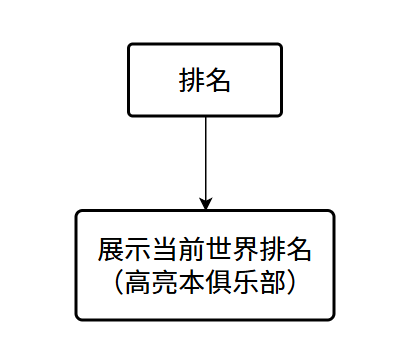
\includegraphics[width=0.5\textwidth]{figure/flowchart/rank.png}
    \end{figure}   
    排名界面中，仅需对俱乐部列表中的俱乐部对象按积分降序排序，并对当前俱乐部高亮即可。


\section{方案拟定和分析}
    程序拟实现的功能如下：
    \begin{enumerate}
        \item 从文件中进行数据的读取和存储
        \item 实现俱乐部的创建和密钥验证
        \item 展示当前俱乐部的信息
        \item 生成并存储各种动态
        \item 用户在市场中进行选手交易
        \item 用户选择赛事进行参与，并反馈比赛结果
        \item 根据积分对当前俱乐部进行排名
        \item 用菜单形式提供程序的各种功能的选择
    \end{enumerate}

\section{实施计划}
\begin{tabular}{c|c}
    %\centering
    \hline
    周数 & 任务 \\ \hline
    第十周 & 学习相关设计模式，新建文件夹，规划好每一部分的文件分配；明确工程规范 \\ \hline
    第十一周 & 拟草UML类图，并建立数据集 \\ \hline
    第十二周 & 完成各类头文件的编写 \\ \hline
    第十三周 & 完成类方法的实现 \\ \hline
    第十四周 & 完成main函数的编写，并进行初步测试 \\ \hline
    第十五周 & 进一步测试完善程序，准备答辩资料 \\ \hline
\end{tabular}

\end{spacing}
\end{document}